%%%%%%%%%%%%%%%%%%%%%%%%%%%%%%%%%%%%%%%%%%%%%%%%%%%%%%%%%%%%%%%%%%%%%%%%%%%%%%%%
\setcounter{section}{0}
%%%%%%%%%%%%%%%%%%%%%%%%%%%%%%%%%%%%%%%%%%%%%%%%%%%%%%%%%%%%%%%%%%%%%%%%%%%%%%%%

\section{科学意义和创新性}

2023年的诺贝尔物理学奖颁发给了Pierre Agostini、Ferenc Krausz和Anne L'Huillier,以
表彰他们``{\kaishu{}将产生阿秒脉冲的实验方法用于研究物质的电子动力学}''。随着超快
激光技术的发展,人们已经有了越来越多的实验技术手段来研究凝聚态体系中的载流子动力
学,诸如时间分辨超快光谱、光电子能谱、甚至时间分辨超快 STM,都给了人们一个全新的、
也就是“时间分辨”的尺度,让人们来理解载流子的动力学行为。然而,由于载流子动力学的
复杂性,只依赖实验的手段人们依然无法有效理解其复杂的、涉及到各种准粒子相互作用的
物理图像,要做到这一点,第一性原理计算这样强有力的工具是必不可少的。我们计划
在\hnamd{}已有的基础上,进一步发展计算方法,实现以下几个目标:

\subsection{基于$GW+{}$BSE计算激发态原子受力,发展针对材料光致相变与材料表面
  光催化反应势垒的计算方法}


当我们考虑载流子的动力学时,材料的原子结构也会受到载流子的影响。例如,在光激发的
条件下,材料有可能发生光致相变,化学分子则有可能通过对电子或空穴的捕获,发生所
谓“光催化”反应。在目前的第一性原理计算领域,研究基态的相变过程以及催化反应势垒已
经有非常成功的方法,\emph{然而针对光致相变与表面分子的光催化反应路径则几乎没有
  研究}。其中的难点就在于如何考虑光激发载流子对晶格及分子结构的影响。

光激发载流子对材料原子结构的影响可以分两方面来考虑:一方面,当电子通过电声散射发
生弛豫时,能量会通过电声耦合传递给相应的声子,产生热效应;另一方面,当电子不是处
于基态,而是在某个“激发态”上的时候,整个晶体的势能面会发生变化。通过电声耦合激发
声子的过程,可以通过计算非绝热耦合或电声耦合来得到,而激发态对势能面的影响,我们
计划通过 $GW+{}$BSE 的计算来获得,这个方案的难点主要在于计算量,在初步进行了一些
推导与测试之后,我们认为可以通过引入一些合理的近似来减少计算量,后续还有可能通过
引入机器学习哈密顿量来进一步降低计算成本,实现实际体系的计算。通过这部分的工作,
我们计划发展一套可实用的算法,可以用于研究光致相变以及表面光催化反应路径。

\subsection{考虑载流子与光场的耦合,发展针对材料发光动力学过程的计算方法}


光场同时也是控制载流子动力学的重要手段。光场与载流子动力学的耦合可以大致分为两个
方面,首先,光场可以激发载流子,人们可以通过控制光子的能量、强度、偏振方向等手段
来控制光激发载流子的能量分布,还可以通过具有手性偏振的光子来控制载流子的自旋;其
次,光场会影响载流子的弛豫过程,电子与空穴可能通过与光场的耦合释放一个光子,发生
辐射复合。在材料发光的过程中,光激发载流子有两条不同的弛豫通道,一条是通过辐射复
合发射光子,而另一条则是通过非辐射复合将能量转移给声子,这两条通道相互竞争,决定
了材料发光的效率,\emph{然而目前并没有合适的第一性原理计算方法来研究}。我们计划
在 \hnamd{} 中加入光场部分,一方面可以用于研究光激发对载流子动力学的调控,另一方
面可以用于研究材料的发光动力学过程,对于发光过程,我们计划给出针对自发辐射与受激
辐射的两种方案。

%%%%%%%%%%%%%%%%%%%%%%%%%%%%%%%%%%%%%%%%%%%%%%%%%%%%%%%%%%%%%%%%%%%%%%%%%%%%%%%%
\section{技术路线}

%%%%%%%%%%%%%%%%%%%%%%%%%%%%%%%%%%%%%%%%%%%%%%%%%%%%%%%%%%%%%%%%%%%%%%%%%%%%%%%%
\subsection{基于$GW+{}$BSE 计算激发态原子受力,发展针对材料光致相变与材料表面}
%%%%%%%%%%%%%%%%%%%%%%%%%%%%%%%%%%%%%%%%%%%%%%%%%%%%%%%%%%%%%%%%%%%%%%%%%%%%%%%%

  \begin{figure}
     \centering
     \captionsetup{width=0.90\textwidth}
     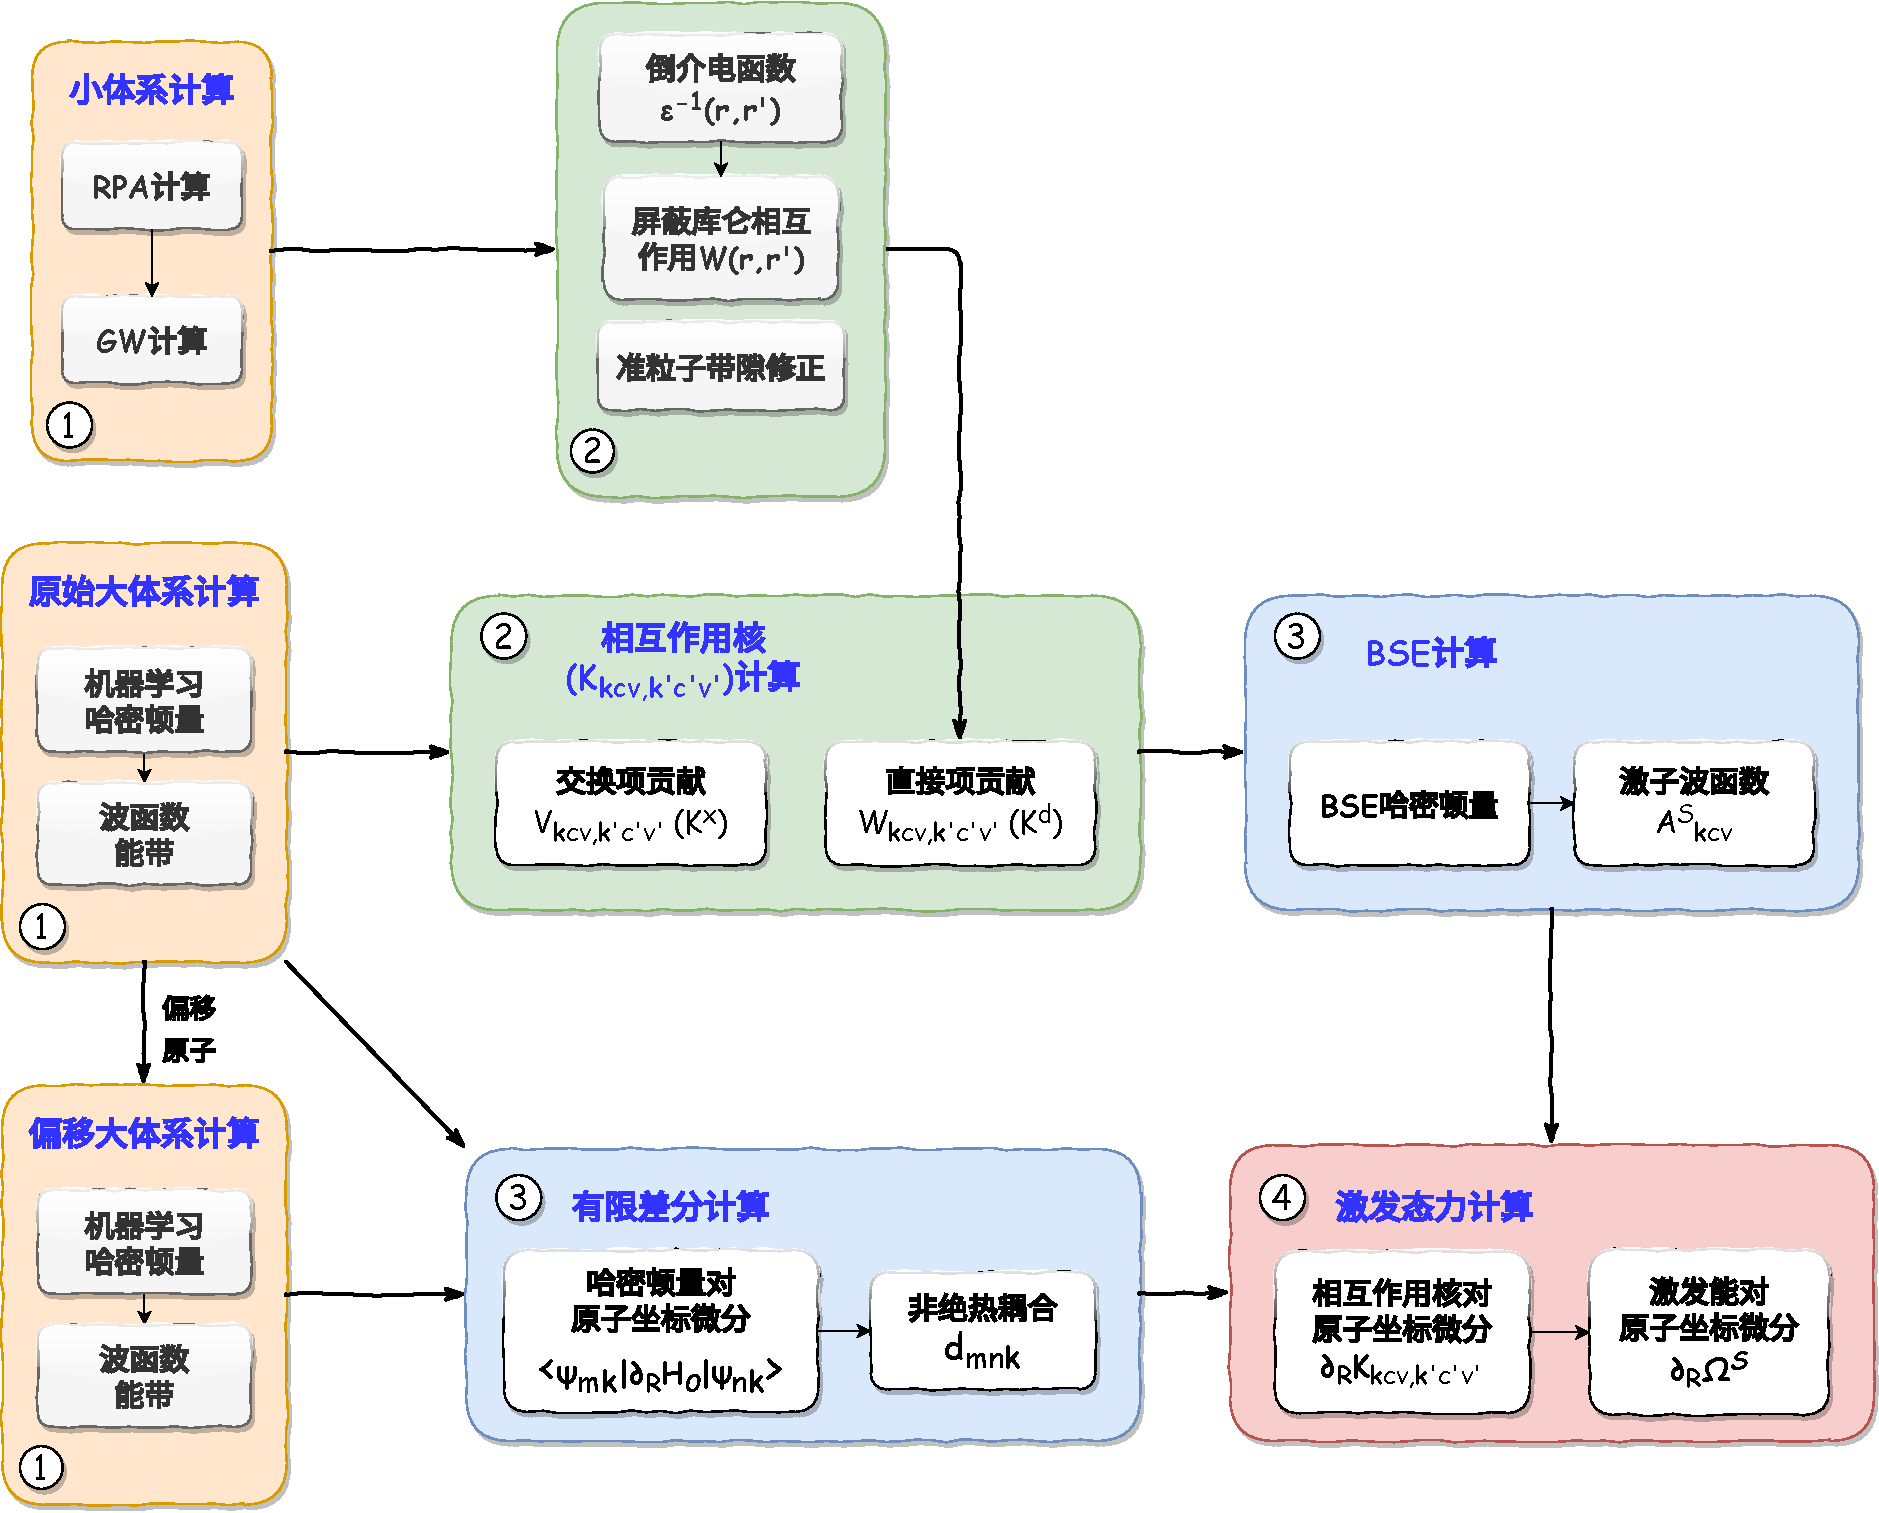
\includegraphics[width=1.0\textwidth]{figs/excited_force_flowchart.pdf}
     \caption{$GW+{}$BSE结合机器学习哈密顿量求解激发态受力的流程示意图。
         \label{fig:excited_force_flowchart}}
  \end{figure}


  固体材料中的原子基态受力可以很容易从DFT理论中得到,由此人们可以对材料结构进行优
  化、并且可以计算一定温度下的分子动力学,以及结构变化的势垒。而固体材料的激发态
  的原子受力则一直是计算的难点,我们借鉴之前在\hnamd{}中实现$GW+{}$rtBSE的思路,
  计划基于$GW+{}$BSE实现激发态原子受力。

  激发态的受力可以用体系总能量对原子坐标的偏微分来表达:
  \begin{equation}
    \partial_\mathbf{R}E_S
    = 
    \partial_\mathbf{R}E_0
    +
    \partial_\mathbf{R}\Omega^S
  \end{equation}
  其中$E_0$是基态能量,而$\Omega^S$是激发能,可以由$GW+{}$BSE得到。此时:
  \begin{equation}
    \partial_\mathbf{R}\Omega^S = \sum_{vc\mathbf{k},v'c'\mathbf{k}'}
    A^{S*}_{vc\mathbf{k}}
    A^S_{v'c'\mathbf{k}'}
    \partial_\mathbf{R}
    H_{vc\mathbf{k},v'c'\mathbf{k}'}^{\mathrm{BSE}}
  \end{equation}
  其中$H_{vc\mathbf{k},v'c'\mathbf{k}'}^{\mathrm{BSE}}$是用来描述激子的哈密顿量,
  对角化之后可以得到激子能量和波函数系数$A^{S}_{vc\mathbf{k}}$。如果我们延
  用$GW+{}$rtBSE中固定介电函数的方法,认为体系的介电函数在空间尺度变化时基本保持
  不变(激子态分布的空间尺度大于介电屏蔽作用范围),那么我们可以通过一次小单
  胞$GW$的计算得到介电函数(或直接基于RPA近似计算介电函数,带隙修正基于将价带或导
  带平移的近似处理,以避免大计算量的$GW$计算),用以构造BSE哈密顿量,并对角化得到
  波函数系数$A^{S}_{vc\mathbf{k}}$。但是,如果我们想通过有限差分的思路得到激发态
  受力,需要对体系中的每一个原子向三个坐标轴方向进行偏移,并计算偏移结构的BSE哈密
  顿量,来求得$ \partial_\mathbf{R}
  H_{vc\mathbf{k},v'c'\mathbf{k}'}^{\mathrm{BSE}} $。这种方案对于原子数较少的体系
  是可以实施的,然而对于原子数较多的体系依然存在计算量过大的问题。

  如果我们把BSE哈密顿量写成如下形式:
  \begin{equation}
    H_{vc\mathbf{k},v'c'\mathbf{k}'}^{\mathrm{BSE}}
    =
    (\varepsilon_{c\mathbf{k}}^{QP} - \varepsilon_{v\mathbf{k}}^{QP})
    \delta_{vv'}\delta_{cc'}\delta_{\mathbf{kk'}}
    +
    K_{vc\mathbf{k},v'c'\mathbf{k}'}
  \end{equation}
  第一项是BSE哈密顿量对角元,通过$GW$准粒子能级构建,第二项是构建BSE哈密顿量所需的
  电子-空穴相互作用核,那么,BSE哈密顿量对原子坐标的微分就可以写成:
  \begin{equation}
    \partial_\mathbf{R}
    H_{vc\mathbf{k},v'c'\mathbf{k}'}^{BSE}
    =
    (\partial_\mathbf{R}\varepsilon_{c\mathbf{k}}^{QP} - \partial_\mathbf{R}\varepsilon_{v\mathbf{k}}^{QP})
    \delta_{vv'}\delta_{cc'}\delta_{\mathbf{kk'}}
    +
    \partial_\mathbf{R}K_{vc\mathbf{k},v'c'\mathbf{k}'}
  \end{equation}
  其中第一项是准粒子能级能量对坐标的微分。如果我们认为准粒子能级的能量相对于DFT
  Kohn-Sham能级的能量只是做了一个平移的话,那么准粒子能量微分项中自能修正的贡献可
  以近似为0,即:
  \begin{align}
    \partial_\mathbf{R}\varepsilon_{n\mathbf{k}}^{QP}
    &= \mel{\psi_{n\mathbf{k}}}{\partial_\mathbf{R} H^{QP}}{\psi_{n\mathbf{k}}}
      = \mel{\psi_{n\mathbf{k}}}{
      \partial_\mathbf{R}
      \left[\hat{T} + \hat{V}_{ion} +
      \hat{V}_H + \hat{\Sigma}\right]}{\psi_{n\mathbf{k}}}
      \nonumber \\
    &= \mel{\psi_{n\mathbf{k}}}{
      \partial_\mathbf{R}
      \left[\hat{T} + \hat{V}_{ion} +
      \hat{V}_{xc}\right]}{\psi_{n\mathbf{k}}}
      +
      {\color{red}
      \mel{\psi_{n\mathbf{k}}}{
      \partial_\mathbf{R}
      \left[\hat{\Sigma} - \hat{V}_{xc}\right]}{\psi_{n\mathbf{k}}}
      (\approx 0)
      }
      \nonumber \\
    &\approx \mel{\psi_{n\mathbf{k}}}{
      \partial_\mathbf{R}
      \left[\hat{T} + \hat{V}_{ion} +
      \hat{V}_{xc}\right]}{\psi_{n\mathbf{k}}}
      \nonumber \\
    &= \mel{\psi_{n\mathbf{k}}}{
      \partial_\mathbf{R} H_0
      }{\psi_{n\mathbf{k}}}
  \end{align}
  其中$H_0$是DFT基态Kohn-Sham哈密顿量,而后面一项为电子-空穴相互作用核对坐标的微
  分,电子-空穴相互作用核矩阵写成:
  \begin{equation}
  K_{vc\mathbf{k},v'c'\mathbf{k'}}=\int{d\mathbf{r}d\mathbf{r'}\psi_{c\mathbf{k}}^{*}(\mathbf{r})\psi_{v\mathbf{k}}(\mathbf{r'})K(\mathbf{r},\mathbf{r'})\psi_{c'\mathbf{k'}}(\mathbf{r})\psi_{v'\mathbf{k'}}^{*}(\mathbf{r'})}
  \end{equation}
  如果考虑其坐标微分,在忽略包含$\partial_\mathbf{R}K(\mathbf{r},\mathbf{r'})$的
  项后,可以推导得到
  \begin{multline}
    \partial_\mathbf{R}K_{vc\mathbf{k},v'c'\mathbf{k}'}  
    \approx
    \sum_n \biggl[
      d^*_{nc\mathbf{k}}K_{vn\mathbf{k},v'c'\mathbf{k}'}  
      +
      d_{nv\mathbf{k}}K_{nc\mathbf{k},v'c'\mathbf{k}'}  
      \\
      +
      d_{nc'\mathbf{k}'}K_{vc\mathbf{k},v'n\mathbf{k}'}  
      +
      d^*_{nv'\mathbf{k}}K_{vc\mathbf{k},nc'\mathbf{k}'}  
    \biggr]
  \end{multline}
  其中$d_{mn\mathbf{k}}$为非绝热耦合项
  \begin{equation}
    d_{mn\mathbf{k}}
    =
    \begin{cases}
      \mel{\psi_{m\mathbf{k}}}{\partial_\mathbf{R}}{\psi_{n\mathbf{k}}}
      =
      \dfrac{
        \mel{\psi_{m\mathbf{k}}}{\partial_\mathbf{R} H_0}{\psi_{n\mathbf{k}}}
      }{
        \varepsilon_{n\mathbf{k}} - \varepsilon_{m\mathbf{k}}
      }, & (m\ne n)
      \\[6pt]
      0, & (m=n)
    \end{cases}
  \end{equation}
  总结一下,如果我们假设准粒子能级相对于Kohn-Sham能级只做一个平移,那么:其中第一
  项中$\partial_\mathbf{R}H_0$是DFT哈密顿量相对于坐标的微分,相当于一个DFPT的计
  算,
  \begin{multline}
    \partial_\mathbf{R} \Omega^S
    =
    \sum_{vc\mathbf{k}}
    |A^S_{vc\mathbf{k}}|^2 \left[
      \mel{\psi_{c\mathbf{k}}}{\partial_\mathbf{R} H_0}{\psi_{c\mathbf{k}}}
      -
      \mel{\psi_{v\mathbf{k}}}{\partial_\mathbf{R} H_0}{\psi_{v\mathbf{k}}}
    \right]
    \\
    +
    \sum_{vc\mathbf{k}, v'c'\mathbf{k}'}
    A^{S*}_{vc\mathbf{k}}
    A^{S}_{v'c'\mathbf{k}'}
    \partial_\mathbf{R} K_{vc\mathbf{k}, v'c'\mathbf{k}'}
  \end{multline}
  后面一项则需要求解BSE方程得到。也就是说,计算一个结构的激发态受力,计算量大约相
  当于一个BSE计算加上一个DFPT的计算。对于DFPT计算,我们可以替代为对原始结构的每个
  原子做偏移,来计算偏移结构的哈密顿量,从而通过有限差分法得
  到$\partial_\mathbf{R}H_0$。如果采用多核并行的方式,可以把针对不同原子平移的计
  算放到不同的核上去进行,从而节省计算时间。这样,预计我们可以处理大约上百个原子
  的体系。后续,我们还计划尝试利用机器学习的方法得到$\partial_\mathbf{R} H_0$,进
  一步降低计算量。图\ref{fig:excited_force_flowchart}中,我们总结了利
  用$GW+{}$BSE求解激发态原子受力的流程。

\subsection{考虑载流子与光场的耦合,发展针对材料发光动力学过程的计算方法}

  \begin{figure}
    \centering
    % \begin{center}
    \captionsetup{width=0.85\textwidth}
    % \includegraphics[width=0.85\textwidth]{figs/namd_emission_flowchart.pdf}
    \includegraphics[width=0.95\textwidth]{figs/namd_emission_flowchart-Page-2.pdf}
    \captionof{figure}{考虑载流子与光场耦合后的 NAMD 流程示意图 
        \label{fig:namd_emission_flowchart}}
    % \end{center}
 \end{figure}


 考虑到载流子与光场的耦合,我们计划在哈密顿量中加入电子与光子的相互作用项:
 \begin{equation}
    \mathcal{H}^{\text{tot}}(\mathbf{r}, \mathbf{R}(t), \sigma, t)
    =
    \mathcal{H}^0 (\mathbf{r}, \mathbf{R}(t)) +
    \mathcal{H}^{\text{ele-phot}}(\mathbf{r}, \mathbf{R}(t), \sigma, t)
 \end{equation}
 其中第一项是体系原有哈密顿量,第二项是电子与光子的相互作用。此时体系的含时演化系
 数方程变为:
 \begin{equation}
 \begin{aligned}
    \frac{\partial c_j(t)}{\partial t}
        &={} \sum_i \left[ i\hbar^{-1} \mel{\psi_j}{\mathcal{H}^{\text{tot}}}{\psi_i} +
            \mel{\psi_j}{\frac{\mathrm{d}}{\mathrm{d}t}}{\psi_i} \right] c_i(t) \\
        &={} \sum_i \left[ i\hbar^{-1} \mel{\psi_j}{\mathcal{H}^0}{\psi_i} +
            i\hbar^{-1} \mel{\psi_j}{\mathcal{H}^{\text{ele-phot}}}{\psi_i} +
            \mel{\psi_j}{\frac{\mathrm{d}}{\mathrm{d}t}}{\psi_i} \right] c_i(t)
 \end{aligned}
 \end{equation}
 如果考虑自发辐射的过程,则电子-光子相互作用可以表示为:
 \begin{equation}
   \mel{\psi_j}{\mathcal{H}^{\text{ele-phot}}}{\psi_i} 
   =
   \frac{e}{m} \sum_{\alpha=1}^3 \sqrt{\frac{\hbar}{2\epsilon_0 \omega_k V}}
   \mel{\psi_j}{e^{-i\omega_{\mathbf{k}}t} \hat{p}_\alpha}{\psi_i} e_{k \lambda}^\alpha.
 \end{equation}
 如果考虑受激辐射过程,则:
 \begin{equation}
 \begin{aligned}
    \mel{\psi_j}{\mathcal{H}^{\text{ele-phot}}}{\psi_i}
        &={} e\mel{\psi_j}{\hat{\mathbf{r}}}{\psi_i} \cdot \mathbf{E}(t) \\
        &={} \frac{ie\hbar}{(\varepsilon_j - \varepsilon_i)m} \mel{\psi_j}{\hat{\mathbf{p}}}{\psi_i} \cdot \mathbf{E}(t).
 \end{aligned}
 \end{equation}
虑了光场之后的程序流程图如图 \ref{fig:namd_emission_flowchart} 所示。


%%%%%%%%%%%%%%%%%%%%%%%%%%%%%%%%%%%%%%%%%%%%%%%%%%%%%%%%%%%%%%%%%%%%%%%%%%%%%%%%
\section{可行性分析}

对于以上几个问题的技术路径我们都做了公式的推导以及仔细的分析,并给出了清晰的执行
路线图,激发态受力的计算涉及到 DFPT 与 BSE 计算,光场的耦合的关键物理量是跃迁偶极
矩。我们已经对计算中关键步骤,例如电声耦合、DFPT、BSE、跃迁偶极等模块进行了测试,
有信心能够顺利完成目标。
%%%%%%%%%%%%%%%%%%%%%%%%%%%%%%%%%%%%%%%%%%%%%%%%%%%%%%%%%%%%%%%%%%%%%%%%%%%%%%%%